\documentclass[oneside]{tudelft-report}
\newcommand{\comment}[1]{}
\usepackage{enumitem}
\usepackage[acronym,nomain]{glossaries} % Load the glossary pacakage with the acronym option
\setlength{\parskip}{1em}
\usepackage[justification=centering]{caption}
\usepackage{pdfpages}
\usepackage{subcaption}

\newcommand{\noop}[1]{} % a do-nothing command that serves a purpose

\begin{document}

%% Use Roman numerals for the page numbers of the title pages and table of
%% contents.
\frontmatter

\title[Final report\\TI3806 - Bachelorproject]{BEPStore}
\author{Bart Heemskerk}{Wouter Kooyman van Guldener}{Steffan Sluis}
\affiliation{Technische Universiteit Delft}
\coverimage{cover2.jpg}
\makecover

%% Include an optional title page.
\input{title}

% Define any acronyms
% Use acronyms with the \gls{} or \Gls{} command
\newacronym{rtc}{RTC}{realtime-clock}
\newacronym{adc}{DAC}{digital-to-analog converter}
\newacronym{dac}{ADC}{analog-to-digital converter}
\newacronym[plural=LEDs,firstplural=light emitting diodes (LEDs)]{led}{LED}{light emitting diode}
\newacronym{spi}{SPI}{serial peripheral interface}
\newacronym{i2c}{I$^2$C}{inter-integrated circuit}
\newacronym{pwm}{PWM}{pulse-width modulation}
\newacronym{tx}{Tx}{transceiver}
\newacronym{rx}{Rx}{receiver}
\newacronym{pwb}{PWB}{printed wiring board}
\newacronym{pcb}{PCB}{printed circuit board}
\newacronym{uml}{UML}{unified modelling language}
\newacronym{mvp}{MVP}{minimum viable product}
\newacronym{sig}{SIG}{Software Improvement Group}
\newacronym{ci}{CI}{Continuous integration}

\chapter*{Preface}
\setheader{Preface}

FeedbackFruits is a company that offers an online learning solution to help innovate education. The platform is used on a daily basis by teachers and students to improve their learning experience. In using the platform, the users often think of valuable feedback and new features they woulld like to see added. This report describes the process of designing and implementing a platform for the puprose of collecting this feedback in a central location and streamline the process of acting upon it.

\begin{flushright}
{\makeatletter\itshape
    \@author \\
    Delft, January 2013
\makeatother}
\end{flushright}


\chapter*{Summary}
\setheader{Summary}

This report describes the process of finding a solution to the problem: ``How can the existing FeedbackFruits platform be extended in such a way that everyone in the FeedbackFruits community can contribute to the software development process?'' This process consist of a research phase and an implementation phase. The conclusions of the research were processed into a set of requirements for a solution. These requirements emphasises the central role of communication in community engagement. Additionally, the research shows that there are no modern tools for requirements engineering, a process centered around decomposing a problem into smaller problems that can be solved in order to find a solution for the bigger problem.

The solution that was implemented during this project facilitates collaboration between technical and non-technical users by integrating existing software development tools and offering their functionalities in an interface that is more user-friendly to non-technical users. Users have the ability to indicate what they would like to see in the FeedbackFruits and share this on social media such as Facebook and Twitter. The solution also provides a centralised means of communication between all supporters of an extension to the FeedbackFruits platform.

The implementation does not cover all of the requirements specified as a result of the research. Although the team would like to have delivered a complete solution, they feel the extensibility of the implementation and the broad scope of the research make up for the requirements that were not implemented during this project.

\tableofcontents

% reset acronyms
\glsresetall

%% Use Arabic numerals for the page numbers of the chapters.
\mainmatter

% Steffan
\chapter{Introduction}

Albert Einstein once said: "I never teach my pupils, I only attempt to provide the conditions in which they can learn." This presents the idea of letting pupils do the learning themselves, as opposed to the traditional idea of a teacher imparting knowledge onto others. This idea has become increasingly popular in recent years with the rise of new methods in education such as 'flip the classroom' and 'blended learning'. Education as an industry seems to be moving towards personalised learning. To offer a personalised learning experience, a set of tools of required that can be adapted to facilitate such an approach. However many tools exist to facilitate the needs of the many, it remains difficult to gain insight into what tools are still missing.

This report describes the process of finding a method for gaining this insight and using it to improve the current state of education. The report is divided into 6 chapters. The first chapter explains the motivation behind the project in the form of a general problem. The second chapter introduces the client and how the general problem concerns them. The third chapter defines the problem in the context of the client. The fourth chapter describes the process used to find a solution to this problem and implement it. The fifth chapter presents the solution and compares it to the implementation. Finally, the sixth chapter presents the results of this comparison and recommendations to improve upon the implementation of the solution.

It is recommended to read the research report (see appendix \ref{app:research_report}) before reading chapters three and onwards. The research report contains valuable background information and is referred to throughout the final report.
% Steffan
\chapter{Client}
The client is FeedbackFruits, a ... company

% Steffan
\section{Needs}

% Steffan
\section{Motivation}
\chapter{Problem}

This chapter gives a description of the problem that was solved over the course of this project. It is divided into two sections. The first section describes the problem that was addressed during this project and the third section gives an analysis of how this problem can be decomposed into smaller problems.

% Wotuer
\section{Problem definition}
In the research report{ref:research-report:v1} a problem description was identified: ``How can the existing platform be extended in such a way that everyone in the FeedbackFruits community can contribute to the software development process?''.

%Wouter
\section{Problem analysis}
The most important aspects to this problem were identified in the research report as being: hype, requirements engineering, code and process updates. 


%Wouter
\chapter{Process}

This chapter describes the specifics of the process followed over the course of this project. It is divided into two section. 


2 week research report, brainstorm,  problem analysis, Scrum, MoSCoW, 
https://www.sharelatex.com/project
\section{Communication}

\section{Research}

%Steffan
% \subsection{Rarareflection dingen}
\section{Solution requirements}
issue 5

\section{Quality Assurance}
Iets over CI, CD, coverage, duplication

\chapter{Solution}

This chapter explains how the solution works for the problem that was described in Chapter 1. It is divided into two sections. The first section gives a formal specification of the solution. The second section shows how this formal specification was implemented over the course of this project.

%Bart
\section{Specification}
It appears that GitHub already implements most of the features needed as specified in the problem analysis. The resulting platform should therefor be an extension to the GitHub platform so it can also be used by non-developers. In the research report a MoSCoW model was proposed \Citep * [chap. 5.5]{research-report:v1.0}

\subsection{Requirements}
MoSCoW

\subsection{Success critera/Use Cases}
% Maybe split this into formal/informal?

\subsection{Definition of Done}
Iets over ons eigen platform gebruiken om zichzelf te ontwikkelen.


\section{Implementation}
% issue 11
Complete description of the final product. %plus graphics

% FlowChart

% UML Diagram

% Plaatje van uiteindelijke platform (?)


% \section{Conclusion}

\chapter{Conclusion}

Over the course of this project, several problems were addressed and solutions were found. This chapter analyses the solution in order to show how and to what extent it solves the problems. The chapter is divided into three sections. The first section draws conclusions about the results of the comparison between the solution and its implementation. The second section gives recommendations for building upon the implemented solution. The third section suggests how the research done for this project might be expanded upon.

\section{Results}

The previous chapter compares the implemented solution with the requirements found during the research phase of the project. In this comparison, the most remarkable differences can be found in the coverage of the different use case that were specified. Of the four use cases, the third and fourth use case could not be fulfilled with the current solution implementation. These use cases are concerned with the share of designs and giving feedback on community contributions. These features were not implemented due to a revision of the planning because of delays.

Looking at the solution requirements it becomes clear that the solution mostly lacks a feedback system. This will have impact on the engagement of the users, because feedback promotes engagement. The reason that these requirements were not fulfilled during the development is also due to the revision of the planning. In the implementation, the issues and milestones are displayed, therefore giving feedback on the process of the goal. To get feedback on the quality of the goal and the work of an individual, the solution must request information about the content of contributions. Doing that in an effective way turned out to be more complicated then originally estimated. GitHub facilitates the feedback in a proper way for the developers, the main users of the feedback. Because of that, it was decided that the feedback about code and quality should remain on GitHub for this version of the solution.

% Steffan
\section{Recommendations}
The most important recommendation is to implement a feedback mechanism as described in the previous section. Such a mechanism would boost the engagement of the platform and increase the ease of determining the value of community contributions.

Additionally, the implemented solution is designed to accommodate integrations with external services. Due to the scope of the project, 
the amount of available integrations is not very large. If the solution is adopted by the client, it is recommended to implement integrations for other services. The integrations that are implemented with the solution focus on the link between developers and non-developers. Because of this, it would be beneficial to focus on integrations with services that target other parts of the software development process, or aspects around it, such as the design of software components.

Furthermore, the implementation of requirements engineering within the solution could be improved. Currently a small layer of extra functionality is added to GitHub issues and milestones. This process could be extended to integrate these issues and milestones better into the solution.

\section{Further research}
The research that was performed over the course of this project unites community engagement with distributed software development, and aims to provide guidelines towards implementing a platform that unites these subjects. It could possibly be expanded upon by finding guidelines for the union of community engagement in other fields and processing these into a general process for stimulating community engagement.

Alternatively, further research could target the more specific forms of community engagement in software development to offer a comparison of the effectiveness of different techniques. The research on community engagement performed over the course of this project offers general guidelines rather than a specific set of instructions or a particular method.

%% Use letters for the chapter numbers of the appendices.
\appendix

\chapter{Original project description}
This chapter contains the problem description as originally formulated by the client. It is divided into the three orignal sections pertaining to the problem, the company and any auxiliary information.

\section{Project description}
Open source software development has grown during past years. With the adoption of Pull Requests as a means of performing code review and Continuous Integration and Continuous Deployment, an interesting model for software development has arisen: crowd-sourced software development.

On the other hand, micro-service oriented application structures have also become popular over the last years. This application architecture often allows for new functionalities to be added with little effort and with decreased risk of unintended consequences, since each part of the application as a whole functions independently. If one part breaks, it doesn't necessarily affect others.

The project consist of building a platform that streamlines the process of building a micro-service that can interact with the FeedbackFruits API. The goal is to allow developers to immediately create new functionalities, with little knowledge about the internal workings of the API. The platform should offer a set of requirements for functionalities, which can be tested for automatically, as well as the ability to request new functionalities, given a set of requirements.

The platform is targeted at developers who are not (completely) familiar with the codebase of the application they are expanding. For that reason, the main goal of the platform should be to streamline the process from feature request to pull request.

During the project, students may encounter the following problems:
\begin{itemize}[nosep]
    \item What kinds of requirements can be automatically tested for, and what kinds can't?
    \item How and when should communication work between platform, developer, feature requester and application maintainers?
    \item How and when does a service become deprecated? How is it maintained?
    \item What feature requests have priority over others, and why?
    \item How does my service communicate with others?
\end{itemize}

\section{Company description}

We are a startup improving education for learners worldwide. Our platform is built on modern web technologies like Rails, Ember.js, HTML5 MongoDB, Elasticsearch and Git. With more than 30K users and a team of over 20 professional geeks, we work to make education better! We are very passionate and dedicated to our mission. Our devteam ranges from students who hack on education part time to full time, full stack, experienced coders. If you would like to join us in making student life better one pull request at a time and want to dig deeper into web building while doing so, keep on reading!

Our product owner, design and development teams work closely together. We work agile using short 2-week release cycles. A number of our developers have done their own graduation projects within FeedbackFruits, while studying at TU Delft. They are well familiar with the process and will be able to give you valuable advice and guidance. Our 2.0 platform on which you would be working is modularized, meaning that you will have significant freedom in choosing the technology you would like to use in your project. 

\section{Auxiliary information}

You will be able to work on the project from our office located in the startup incubator Yes!Delft. This will allow you to experience the awesome atmosphere in the startup community and being around some of the most innovative businesses in Europe. You will be renumerated for the work on your project and will enjoy all the awesome free lunches, weekly dinners, and other team events like sailing trips and prison breaking.

Our team consists of both dutch and international people, therefore, you will be able to write your proposal in the preferred by you language (Dutch or English). We do not oppose any limitations as to the group size, but would recommend a group size of 2-3 people. One student (R.S. Sluis) has already confirmed his participation in this project.

Last but not least you will have the opportunity to be coached by Emile Hendriks, the director of Computer Science education at TU Delft. Emile has published over 100 papers in international journals and conferences and has supervised over 50 master students and co-supervised 10 PhD students and is one of the leading educational visionaries in the Netehrlands. .
\chapter{Solution Requirements}\label{app:solution_req}

In the initial research report\footnote{\url{https://bep-store.gitbooks.io/research-report/content/v/f60f68494dba238334cb22dc076b64b55bbae851/}} a MoSCoW model \Citep{moscow2014} was proposed as the requirements for the platform. The following requirements are the proposed requirements, separated by must-have, should-have, could-have and won't-have. 

\section*{A user of the platform must be able to:}
\begin{itemize}[nosep]
    \item See a landing page
    \item create a account
    \item view a list of goals
    \item create a goal
    \item join a goal as core team member
    \item see a goals description
    \item see a list of (sub-)challenges for a goal
    \item prioritise (sub-)challenges
    \item use GitHub integrated
    \item decompose a goal into (sub-)challenges in a structured way \Citep {hoffmann2004requirements}
    \item get the following information about a goal:
        \begin{itemize}
            \item progress
            \item milestones/challenges
            \item quality
        \end{itemize}
    \item get feedback on his/her work (via peer review)
    \item give feedback on the work of another user
    \item communicate with other users
\end{itemize}
\section*{A user of the platform should be able to:}
\begin{itemize}[nosep]
    \item have a general information page
    \item join a goal as a contributor
    \item set estimated necessary resources for a goal
    \item set estimated necessary tags for a goal
    \item edit a goal he/she owns
    \item view a list of newest goals
    \item search/browse for goals
    \item hype his/her goals by sharing it on social media
    \item get the following information about a goal:
        \begin{itemize}
            \item a timeline
            \item the functionality
        \end{itemize}
    \item get feedback on his/her work via automated testing
    \item communicate with other users via different tools 
    \item get updates via push-notifications, e-mail etc.
    \item see his/her contributions
\end{itemize}
\section*{A user of the platform could be able to:}
\begin{itemize}[nosep]
    \item edit his/her account
    \item be able to join a project as a backer
    \item view a list of trending goals
    \item get the following information about a goal:
        \begin{itemize}
            \item bounty
            \item availible resources
            \item hype factor
        \end{itemize}
    \item get reputation
    \item view the reputation of a user
    \item be engaged through gamification
    \item follow a tutorial on how to use the platform
    \item get tips on how to use the platform
\end{itemize}
\section*{A user of the platform won't be able to:}
\begin{itemize}[nosep]
    \item follow a tutorial on how to use the platform, based on the type of user
    \item join a training party
    \item take part in a ranking system
    \item be matched with an apprentice
    \item be matched with a senior
\end{itemize}
\chapter{Infosheet}
\begin{description}[nosep]
    \item[Title of the project:] The reverse app store
    \item[Client:] L.\ Starovoitova, FeedbackFruits
    \item[Coach:] Dr.\ E.A.\ Hendriks, Opleidingsdirecteur, Computer Science, TU Delft
    \item[Contact person:] W.J.\ Kooyman van Guldener, \url{wouter@wick-it.nl}
    \item[Final presentation date]: June 24th, 2016
\end{description}

\section{Description}
% \subsection{Challenge}
Engagement of non-technical users in the software development process is difficult. Users often have valuable feedback on the clients platform, but the real value of their feedback often gets lost in the translation to the actual software implementation. 

% \subsection{Research}
The requirements for community engagement have been thoroughly researched, with a focus on software communities. Additionally, requirements engineering was also researched to gain insight into feedback aggregation and problem decomposition.

% \subsection{Process}
The team adopted an agile approach for creating an optimal solution in a short period. Many tools were used to ensure a stable production environment and a good code climate. Because the team was based at the client, continuous input of the client made it possible to fully customise the solution to the clients needs.

% \subsection{Product}
The implemented solution is a platform that is closely connected to the clients platform, focused on engaging non-technical users in the process of enhancing the clients platform. With the solution it is possible to create a goal. Through GitHub integration it is possible to create issues and milestones in a readable format for non-technical users. It is also possible to share a goal via Twitter, Facebook and LinkedIn. Communication is provided via Gitter integration. The solution is live\footnote{\url{https://bepstore.feedbackfruits.com}} and will be subjected to a user test in the form of a hackathon.

% \subsection{Outlook}
While the current solution is already live, it can still be improved. A future version of the platform would add more integrations and make it even more easy for users to engage. Focus should be on an improved version of the requirements engineering part and involvement of designers.

\section{Most important contributions per project member}
\begin{description}
    \item[Bart Heemskerk] Responsible for the larger part of the design and usability of the front-end.
    \item[Wouter Kooyman van Guldener] Responsible for the larger part of the back-end and synchronisation between users.
    \item[Steffan Sluis] Responsible for the integration of external services and compatibility with the client's platform.
    \item[All] Responsible for the research report, final report, final project presentation and quality assurance.
\end{description}

“The final report for this project can be found at: 
        "\url{http://repository.tudelft.nl}"


% The Info sheet is a single A4 that contains a description of the project, including information on 
% its unique points, and a short blurb on the role of each of the team members. It should contain the 
% following points: 
% - Title of the project 
% - Name of the client organization 
% - Date of the final presentation 
% - Description 

% Short description of the problem that was tackled by the project, including one or two lines about the client. You may also add a diagram, photo or logos (e.g., TU Delft Logo). Note: if the problem formulation shifted or developed over the course of the project, describe the problem that was actually addressed, and not the problem that was initially intended to be addressed. Please briefly touch on each of these points in your description: 

%     -  Challenge: Statement of the core challenge of the project. 
%     - Research: Statement of what the students learned during the research phase, and how 
%     that informed the decisions in the project. 
%     - Process: Statement of how the process was set up, and any adaptations that needed to be 
%     made while the process was running. Mention (briefly!) any unexpected challenges  and 
%     how they were overcome. 
%     - Product: Description of the product that was created, and how it was tested. 
%     - Outlook: Describe the outlook of the product. Did the team make recommendations to the     client? (if so, briefly summarize) Will the product be used?  
    
    % Members of the project team 
    % For each team member include: 
    % - Name (nB do not include student numbers.) 
    % - One sentence description of the person’s interests (including and going beyond computer science, if relevant) and (optional) of any other relevant facts about experience. (If you really don’t want to list interests, then you can skip this sentence, if you have many, then you can add two sentences.) 
    % - Description of the contributions of the person to the project, and the role played by that person in the project. Be sure to highlight the critical contributions. 
    % If there is something that all team members did, that can be included as a separate sentence at the bottom (in order to avoid redundancy): e.g., “All team members contributed to preparing the report and the final project presentation”. 
    % Please include this information at the bottom of the page: 
    % - Name and affiliation of the Client 
    % - Name and affiliation (Department and Group) of the TU Coach 
    % - Contact person: The email address of one or more people (team members or project 
    % coach) to contact that is expected to be valid at least five years after the completion of the 
    % project. 
    % -  The sentence 
 
% We provide some early examples of Infosheets to convey an idea of what they should contain. 
% Note that these are not necessarily complete or optimal, but rather provide the team with an idea 
% of how to create their own. 
% http://homepage.tudelft.nl/q22t4/Resources/TUDelftCSBachelorProjectInfosheetExamples.pdf 
\chapter{Research Report}\label{app:research_report}

This chapter includes the final version of the research report. It describes the problem that was solved during this project, the research questions associated with this problem and the conclusions to these questions based on the research that was performed. It should be noted that section 5.5 of the research report contains a revised version of the solution requirements. The orignal version of the solution requirements is included in appendix B.

\includepdf[pages=-]{./media/research-report.pdf}
\chapter{Conceptual Solution}\label{app:brainstorm1}
Figure \ref{fig:brainstorm} shows the results of the most important brainstorm session at the start of the project.
\begin{figure}[ht]
    \centering
    \includegraphics*[width=\textwidth]{./media/brainstorm}
    \caption{Result of the most important brainstorm session}
    \label{fig:brainstorm}
\end{figure}


\chapter{\texorpdfstring{\Gls{sig}}{SIG} Feedback}
There are two checks performed by \gls{sig}. The feedback for the first check was in Dutch and has been translated. The results for the second check have not yet been received so could not be processed.

\section{Feedback content}
The code of the system scores 4.5 stars on our maintainability-scale, which means that the maintainability of the code is above average. However, improvements can be made when it comes to duplication.

Duplication is determined by looking at the percentage of code which is redundant, primarily the code that has multiple occurrences in the system and can be removed. From the perspective of maintainability, it is desirable to have a low percentage of redundancy, because adjustments to the redundant code have to be done in multiple places.

Multiple duplications are found in the code. For example, the file \textit{click-outside.js} is present two times in the implementation. Duplication was found between the files \textit{show.js}, \textit{edit.js} and \textit{deploy.js}. In the html-code (\textit{422.html}, \textit{404.html} and \textit{500.html}) duplication also occured. The same 45 lines of code are present in all three locations. Try to rewrite the code in a easier way, such that the code can be reused instead of duplicated.

Finally it is good to see that you have written a lot of test-code besides the production-code. The ratio of test-code and production-code is 2:3.

We hope that you are able to maintain the quality of the code as well as the ratio of test-code and production-code during the remainder of the project.''

\subsection{Processing of feedback}
The feedback indicates that the structure of the implementation is good. \Gls{sig} is satisfied with the ratio of test-code and production-code. Combined with the test coverage aggregated by CodeCov, the end-product will be well-tested.

The only negative comments are about code duplications. While the duplication in the html-code were auto-generated by \textit{Ruby on Rails}, they were corrected nonetheless.

The other duplications were in the files \textit{show.js}, \textit{edit.js} and \textit{deploy.js}. However, after investigation it was concluded that \textit{deploy.js} was misspelled and should actually have been \textit{destroy.js}. To remove most of the duplication, the recurring parts were combined into its own function. Part of the duplication is caused by simple import statements. It does not make sense to refactor those.

\subsection{After the feedback}
After the feedback was received, the team was more keen on spotting and avoiding code duplication in (each others) pull requests. Pull requests were only merged if the duplication was removed. According to CodeClimate the \textit{Rails-api} has no duplications at all, and the \textit{Ember-ui} indicates that there are two small duplications. The fixes for these duplications make the code less readable, so it has been decided to not remove those duplications.

% De code van het systeem scoort 4.5 ster op ons onderhoudbaarheidsmodel, wat betekent dat de code bovengemiddeld onderhoudbaar is. Er zijn echter een paar verbeteringspunten bij Duplication.

% Voor Duplicatie wordt er gekeken naar het percentage van de code welke redundant is, oftewel de code die meerdere keren in het systeem voorkomt en in principe verwijderd zou kunnen worden. Vanuit het oogpunt van onderhoudbaarheid is het wenselijk om een laag percentage redundantie te hebben omdat aanpassingen aan deze stukken code doorgaans op meerdere plaatsen moet gebeuren. 

% Er zijn in dit project meerdere duplciaties te vinden: bijvoorbeeld het click-outside.js bestand is twee keer in de upload aanwezig. Verder is duplicatie gevonden tussen de bestanden show.js, edit.js en deploy.js. Ook in de html code (422.html 404.html, 500.html) is de code gekopieerd, dezelfde 45 lines of code zijn aanwezig op alle drie verschillende locaties. Probeer deze code te herschrijven op een slimmere manier, zodat de code wordt hergebruikt in plaats van gedupliceerd. 

% Tot slot is het goed om te zien dat jullie naast productiecode ook redelijk veel testcode hebben geschreven. De verhouding tussen testcode en productiecode is 2:3. 

% Hopelijk lukt het jullie nog om zowel de kwaliteit van de code als de verhouding tussen testcode en productiecode tijdens het vervolg van het project te behouden.
\chapter{Reflection}

\section{Process}

\section{Product}

\section{Challenges}
Iets over de FBF stack en micro-services (veel repos)
\chapter{Design and implementation}

This chapter compares the designs that were made over the course of the project to that of the solution implementation. The designs that are compared are that of the goals, issues and chat. These cover the most important aspects of the platform: collaborative innovation, problem decomposition and communication.

\section{Goals}

\begin{figure}[ht!]
    \centering
    \begin{subfigure}[b]{0.45\textwidth}
        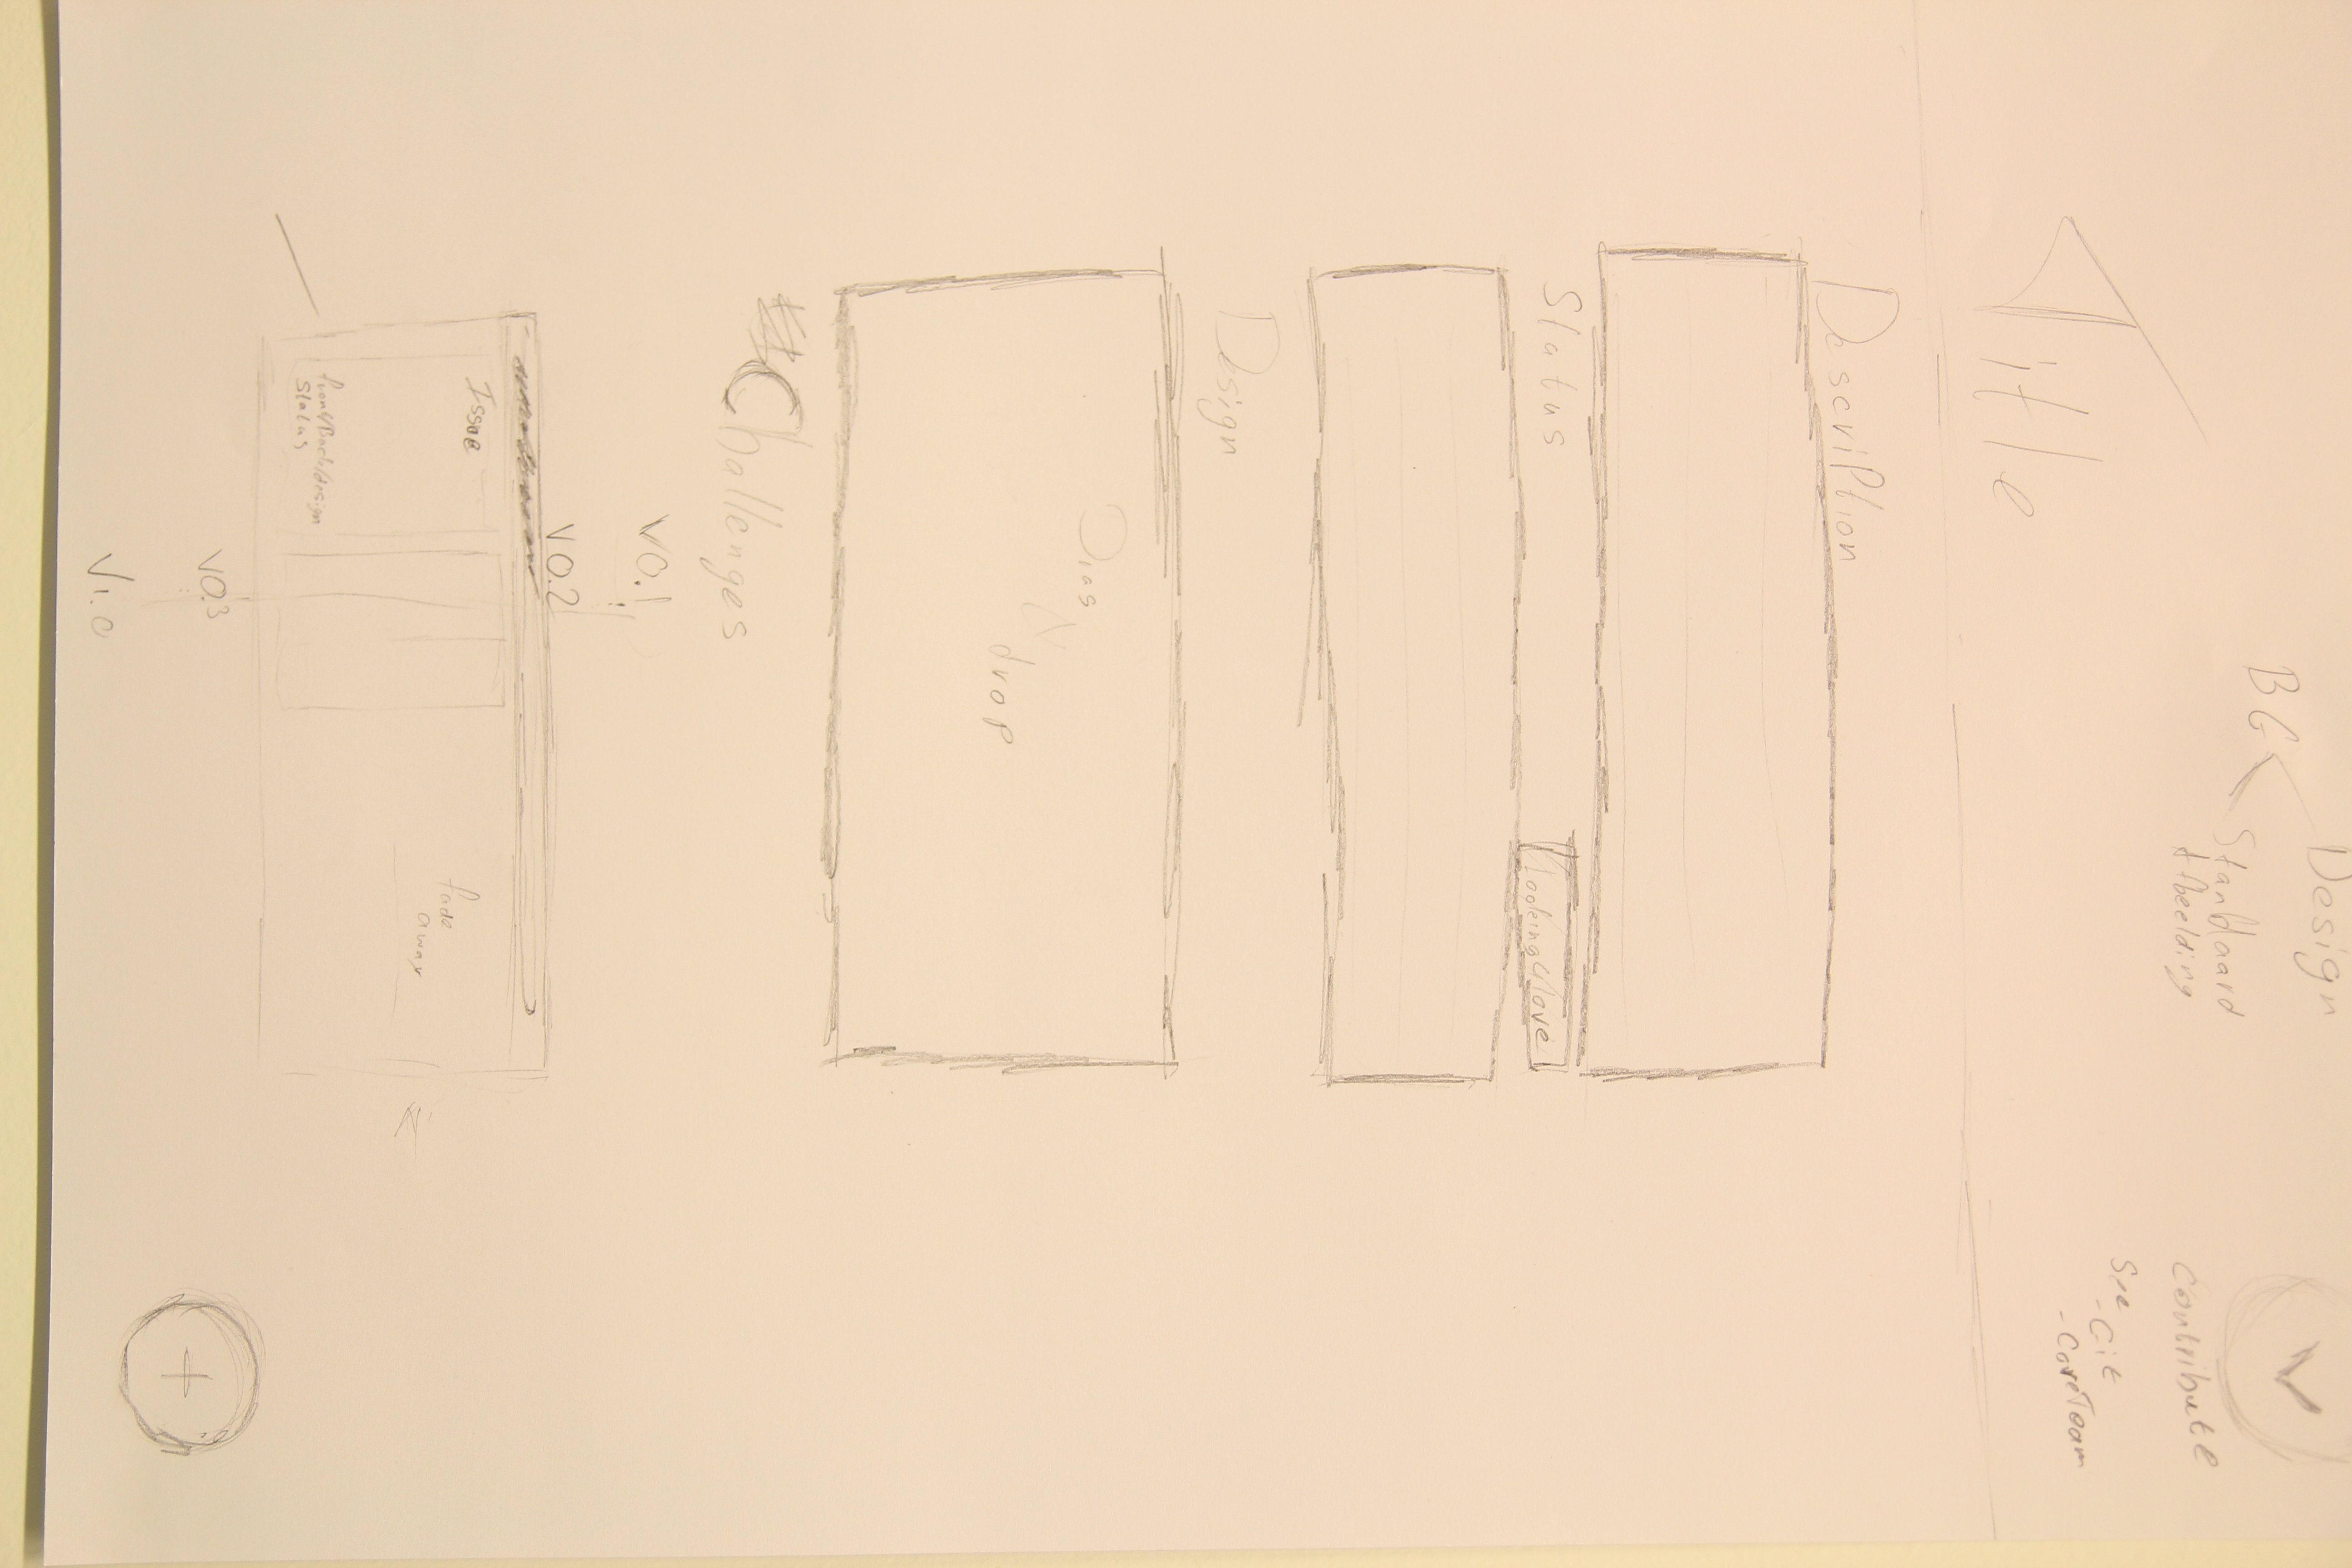
\includegraphics[height=\textwidth, angle=90]{./media/goal_design}
        \caption{The design for viewing a single goal}
        \label{fig:goal-design}
    \end{subfigure}
    ~ %add desired spacing between images, e. g. ~, \quad, \qquad, \hfill etc. 
      %(or a blank line to force the subfigure onto a new line)
    \begin{subfigure}[b]{0.45\textwidth}
        \centering
        \includegraphics[width=\textwidth, height=0.45\textheight, keepaspectratio]{./media/goal_implementation}
        \caption{The implementation for viewing a single goal}
        \label{fig:goal-implementation}
    \end{subfigure}
\end{figure}
\clearpage
\section{Issues}

\begin{figure}[ht!]
    \centering
    \begin{subfigure}[b]{0.45\textwidth}
        \centering
        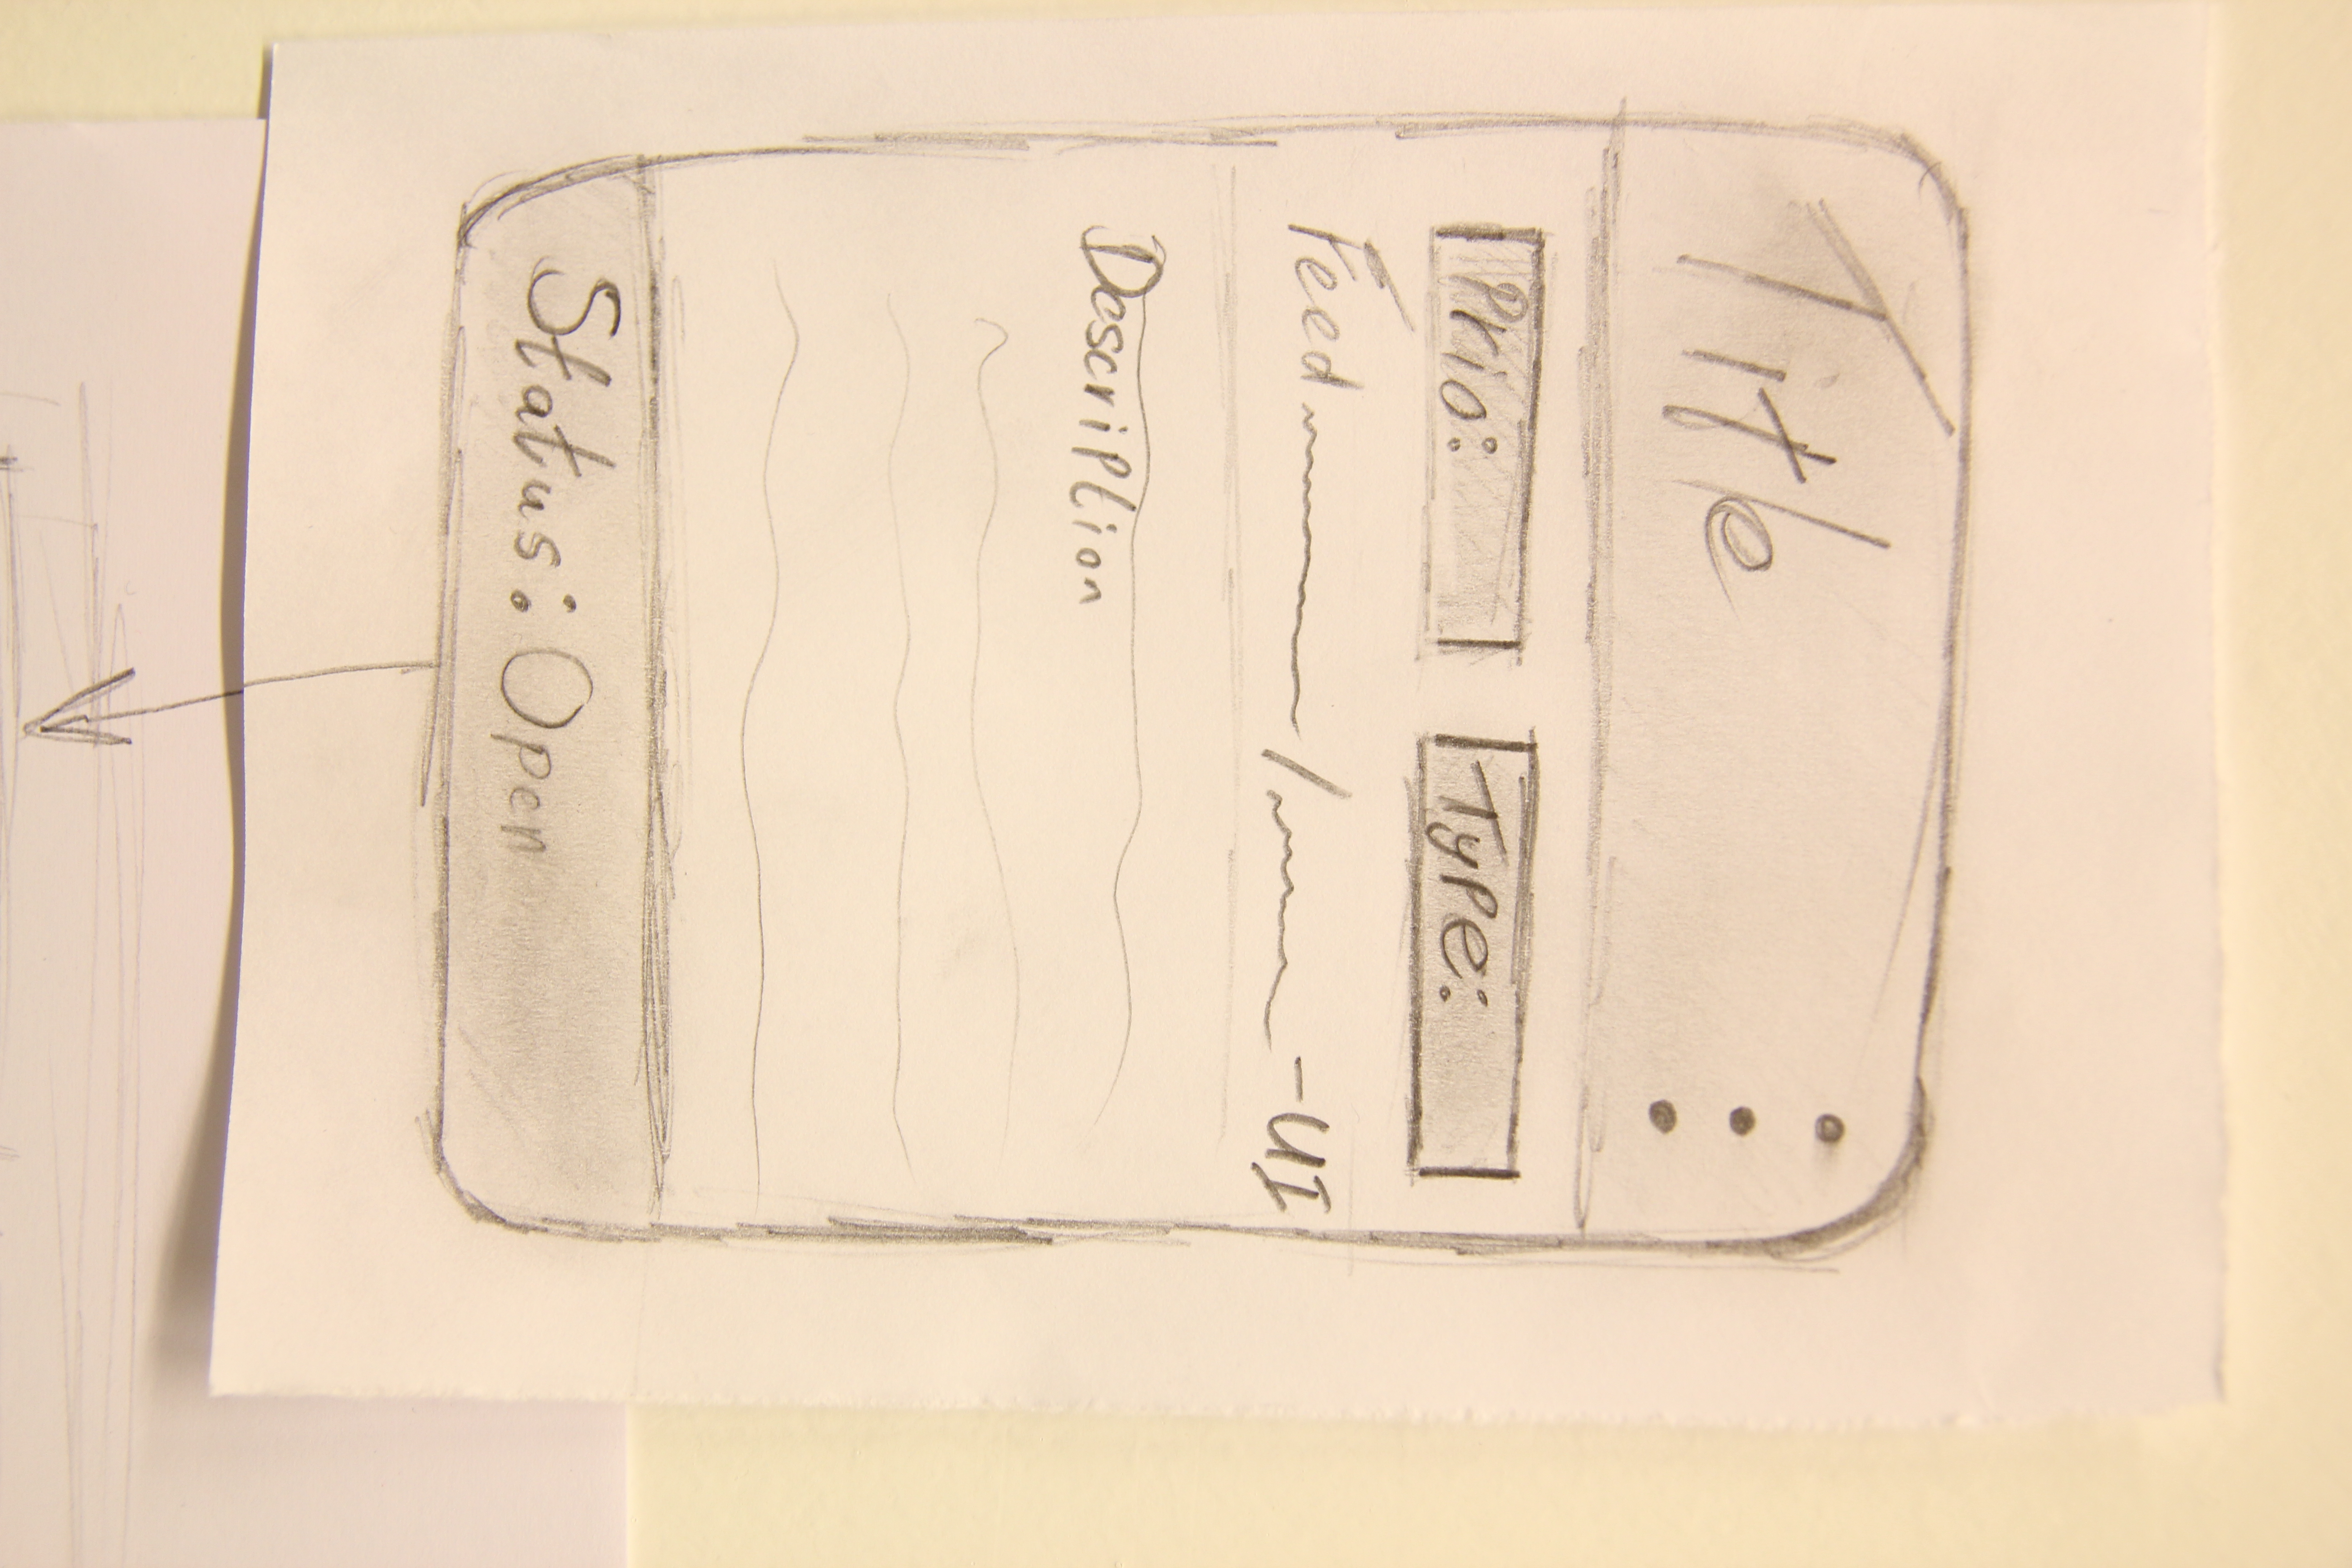
\includegraphics[height=0.75\textwidth, angle=90]{./media/issue_design}
        \caption{The design for viewing a single issue}
        \label{fig:issue-design}
    \end{subfigure}
    ~
    \begin{subfigure}[b]{0.45\textwidth}
        \includegraphics[width=\textwidth]{./media/issue_implementation}
        \caption{The implementation for viewing a single issue}
        \label{fig:issue-implementation}
    \end{subfigure}
\end{figure}

\section{Chat}

\begin{figure}[ht!]
    \centering
    \begin{subfigure}[b]{0.45\textwidth}
        \centering
        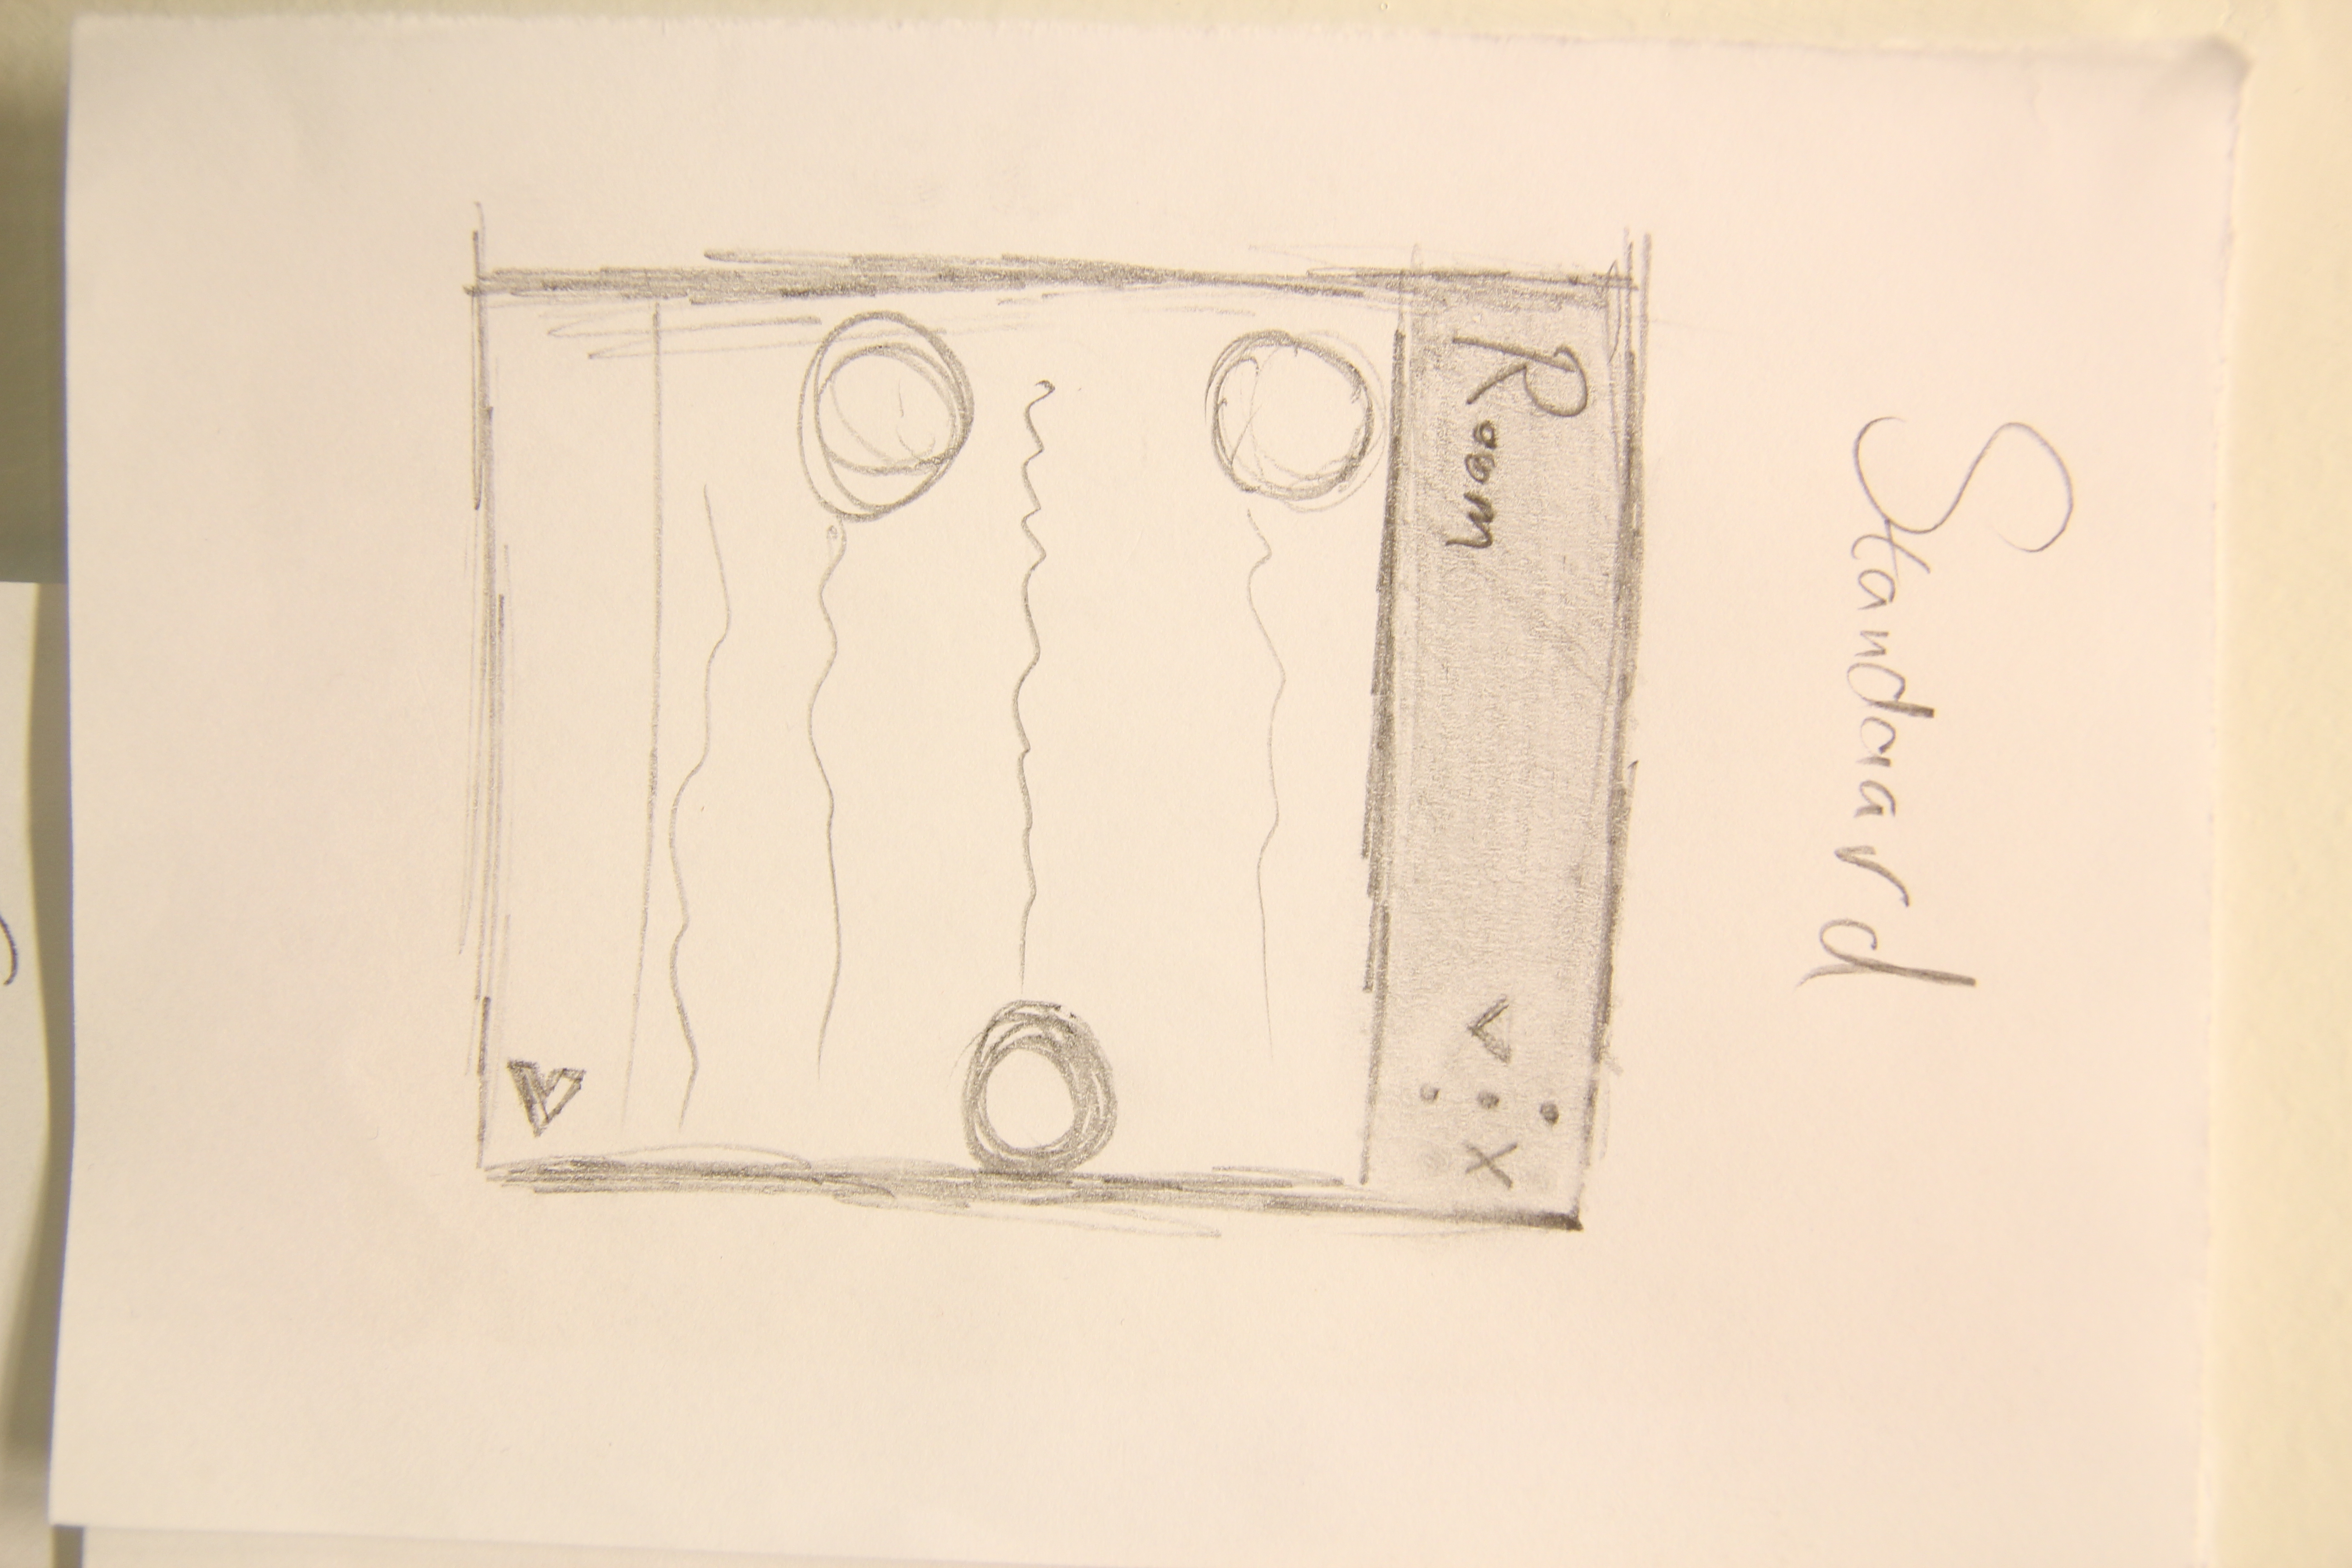
\includegraphics[height=0.75\textwidth, angle=90]{./media/chat_design}
        \caption{The design for viewing the chat}
        \label{fig:chat-design}
    \end{subfigure}
    ~
    \begin{subfigure}[b]{0.45\textwidth}
        \includegraphics[width=\textwidth]{./media/chat_implementation}
        \caption{The implementation for viewing the chat}
        \label{fig:chat-implementation}
    \end{subfigure}
\end{figure}


\bibliography{report}

\end{document}

